\documentclass{thesisclass}
% Based on thesisclass.cls of Timo Rohrberg, 2009
% ----------------------------------------------------------------
% Thesis - Main document
% ----------------------------------------------------------------
\usepackage{algorithm}
\usepackage{algpseudocode}
\usepackage{amsmath}
\usepackage[babel,german=quotes]{csquotes}
\usepackage{csvsimple}
\usepackage{pgfplots}

%% -------------------------------
%% |  Information for PDF file   |
%% -------------------------------
\hypersetup{
 pdfauthor={Dominic Rausch},
 pdftitle={Breitensuche in X10},
 pdfsubject={Breitensuche in X10},
 pdfkeywords={Breitensuche, BFS, breadth-first search, bachelorarbeit, bachelor thesis, Dominic Rausch }
}


%% ---------------------------------
%% | Information about the thesis  |
%% ---------------------------------

\newcommand{\myname}{Dominic Rausch}
\newcommand{\mytitle}{Parallele Breitensuche\\ 
											in X10}
\newcommand{\myinstitute}{Institute for Program Structures\\
													and Data Organization (IPD)}

\newcommand{\reviewer}{Prof. Gregor Snelting}
\newcommand{\advisor}{Andreas Zwinkau}

\newcommand{\timeend}{1. Oktober 2012}
\newcommand{\submissiontime}{1. 10. 2012}



%% --------------------------------
%% | Settings for word separation |
%% --------------------------------
% Help for separation:
% In german package the following hints are additionally available:
% "- = Additional separation
% "| = Suppress ligation and possible separation (e.g. Schaf"|fell)
% "~ = Hyphenation without separation (e.g. bergauf und "~ab)
% "= = Hyphenation with separation before and after
% "" = Separation without a hyphenation (e.g. und/""oder)

% Describe separation hints here:
\hyphenation{
% Pro-to-koll-in-stan-zen
% Ma-na-ge-ment  Netz-werk-ele-men-ten
% Netz-werk Netz-werk-re-ser-vie-rung
% Netz-werk-adap-ter Fein-ju-stier-ung
% Da-ten-strom-spe-zi-fi-ka-tion Pa-ket-rumpf
% Kon-troll-in-stanz
}


%% ------------------------
%% |    Including files   |
%% ------------------------
% Only files listed here will be included!
% Userful command for partially translating the document (for bug-fixing e.g.)
\includeonly{%
titlepage,
declaration,
introduction,
content,
evaluation,
conclusion,
appendix
}


%%%%%%%%%%%%%%%%%%%%%%%%%%%%%%%%%
%% Here, main documents begins %%
%%%%%%%%%%%%%%%%%%%%%%%%%%%%%%%%%
\begin{document}

% Remove the following line for German text
%\selectlanguage{english}

\frontmatter
\pagenumbering{roman}
\include{titlepage}
%!TEX root = thesis.tex

\vspace*{36\baselineskip}
\hbox to \textwidth{\hrulefill}
\par
\iflanguage{english}{I declare that I have developed and written the enclosed thesis completely by myself, and have not used sources or means without declaration in the text.}{Ich versichere wahrheitsgem\"a\ss, die Arbeit selbstst\"andig angefertigt, alle benutzten Hilfsmittel vollst\"andig und genau angegeben und alles kenntlich gemacht zu haben, was aus Arbeiten anderer unver\"andert oder mit Ab\"anderungen entnommen wurde.}

\textbf{Karlsruhe, 1. Oktober 2012}
\vspace{1.5cm}

\dotfill\hspace*{8.0cm}\\
\hspace*{2cm}(\textbf{Dominic Rausch}) %center name with hspace

\thispagestyle{empty}
\blankpage


%% -------------------
%% |   Directories   |
%% -------------------
\tableofcontents
\blankpage


%% -----------------
%% |   Main part   |
%% -----------------
\mainmatter
\pagenumbering{arabic}
%!TEX root = thesis.tex
%% ==============================
\chapter{Einleitung}
\label{ch:einleitung}
%% ==============================

% Kurze BFS Vorstellung
Die Breitensuche (engl: Breadth first search, kurz BFS) ist einer der Standardalgorithmen zur Graphtraversierung. Ausgehend von einem Knoten, dem Wurzelknoten, werden alle transitiv erreichbaren Knoten gesucht Zu jedem der erreichbaren Knoten kann außerdem die Distanz, gemessen in Kantenanzahl, oder der Vorgängerknoten ausgegeben werden. Die Breitensuche findet Anwendung, wenn der kürzeste Weg von einem Knoten zu allen anderen berechnet werden soll. Der von der Breitensuche erzeugte Schichtengraph wird zum Beispiel in Dinic's Algorithmus zur Lösung des Max-Flow Problems wie in \cite{Dinitz:2006} verwendet. 

% Geschwindigkeit durch Parallelität
Lange Zeit wurden Geschwindigkeitssteigerungen der Computer vor allem durch erhöhte Taktraten erreicht. Der Intel 4004 Chip von 1971 taktete mit 108kHz, der 2002 eingeführte Pentium M schon mit 1.7 GHz. 2005 führte Intel den ersten echten Mehrkernprozessor ein(\cite{Intel:2006:Online}), der zwei vollständige Kerne auf einem Chip vereinte. Über 30 Jahre lang optimierte man Prozessoren darauf, einen einzelnen, sequentiellen Befehlsstrang möglichst schnell ausführen zu können. Da aber kein Wechsel des Paradigmas stattfand, skalierten vorhandene Anwendungen sehr gut mit der Geschwindigkeit der Prozessoren. Seit einigen Jahren ist aber klar, dass weitere Geschwindigkeitssteigerungen nur durch (massive) Parallelität geschehen können.  

% Keine unabhängigen Fäden möglich
Die Breitensuche ist ein einfacher Algorithmus, dessen sequentielle Version in ein paar Zeilen Code ausgedrückt werden kann. Das Problem bei der Anpassung an parallele Programmierparadigmen ist, dass keine voneinander unabhängigen Aufgaben für einzelne Bearbeitungsfäden definiert werden können. Sowohl Daten- als auch Kontrollfluss müssen teuer synchronisiert werden.

% Überblick über die Arbeit
% TODO: Überblick über die Arbeit schreiben

Ziel:
Das Paper von \cite{Buluc:2011} beschreibt Ansätze zur Parallelisierung der Breitensuche. Dabei werden zur Kommunikation vor allem MPI Operationen eingesetzt. Wie die Autoren des Papers bereits bemerken, bleibt die Frage offen, ob die vorgeschlagenen Konzepte auch mit modernen, implizit parallelen, Programmiersprachen funktionieren und performant sein können, da eine abstraktere Beschreibungssprache meistens weniger flexibel ist und etwas mehr Overhead benötigt. Weiter soll erforscht werden, wie die Breitensuche mit den Besonderheiten des Inasiven Rechnens zurecht kommt. Dabei sei vor allem die Asymmetrie der Rechenleistung erwähnt, das heißt, einzelne Prozesse haben zum Teil bedeutend mehr Rechenleistung als andere.
%!TEX root = thesis.tex
%!TEX root = thesis.tex
\chapter{Grundlagen} % (fold)
\label{cha:grundlagen}

\section{Die Programmiersprache X10} % (fold)
\label{sec:die_programmiersprache_x10}
Die Programmiersprache X10 wird seit 2004 am IBM T. J. Watson Research Center bei New York in Kooperation mit einigen Universitäten entwickelt und gepflegt. X10 ist eine stark und statisch typisierte, objektorientierte Programmiersprache ohne Mehrfachvererbung. Was sequentielles Programmieren betrifft, entspricht die Feature-Liste weitgehend denen, die von anderen modernen objektorientierten Sprache bekannt sind. Nach Aussage der Entwickler ist X10 im Moment vor allem noch ein Forschungsobjekt und noch nicht für den Produktiveinsatz geeignet. Das Forschungs- und Entwicklungsziel von X10 ist es, eine Abstraktion von paralleler Programmierung zu finden, die es dem Entwickler erlaubt produktiver zu sein, als es mit traditionelleren Sprachen wie Java möglich wäre. Dazu wurden der Programmiersprache Konstrukte hinzugefügt, die einen impliziteren Umgang mit Parallelismus erlauben. Das Programmiermodell folgt dem PGAS (Partitioned Global Address Space) Speichermodel. Die drei für das Verständnis wichtigsten Aspekte von X10 sollen hier kurz beschrieben werden.\cite{x10FAQ:2012:Online}

\subsection{Activities und das Keyword \textit{async}}  % (fold)
\label{sub:aktivitaeten_und_das_keyword_async}
Das Konzept der \textit{Activity} in X10 ist dem der Threads sehr ähnlich. Eine Activity hat einen Programmzähler, einen eigenen Stack und ist semantisch nebenläufig zu allen anderen Activities. Jede Activity lebt zu einem Zeitpunkt auf genau einem Place. Beim Programmstart wird automatisch eine Activity gestartet, die bei der main-Methode beginnt. Mehrere Activities rechnen also potentiell parallel. Tatsächlich werden alle Activities aus einem Threadpool versorgt, der für den Programmierer aber vollkommen transparent ist. Die Laufzeitumgebung von X10 weißt den Threads aus dem Pool nach einer eigenen Policy Activities zu, was vom Programmierer nicht direkt beeinflusst werden kann. Eine neue Activity kann ausschließlich mit dem Keyword \textit{async} gestartet werden. \textit{ async x = calculateX();} führt nebenläufig \textit{calculateX()} aus und weist \textit{x} dann das Ergebnis zu. Um auf die Fertigstellung zu warten, gibt es das Keyword \textit{finish\{...\}}, auf das ein Codeblock folgt. Bevor eine Activity einen finish-Block verlässt, wartet sie, bis alle (auch transitiv) von dieser Activity durch \textit{async}s in diesem Block gestarteten Activities beendet wurden.\cite{x10Spec:2012:Online}
% subsection das_keyword_textit_async (end)

\subsection{Places und das Keyword \textit{at}} % (fold)
\label{sub:places_und_das_keyword_at}
Ein Place in X10 ist die Abstraktion eines Prozessors oder eines Prozessorkerns, auf dem gerechnet werden kann. Zwei unterschiedliche Places haben keinen gemeinsamen Speicher. Um zwischen Places zu wechseln und zu kommunizieren erfolgt kein explizites Message Passing. Stattdessen gibt es das Keyword \textit{at(place) \{ /* code */ \}}. Mit \textit{at} wechselt die aktuelle Activity den Place. Der Code innerhalb des \textit{at}-Blockes wird auf dem entfernten Place ausgeführt. Dazu werden bei jedem \textit{at} alle Objekte, die innerhalb des Blockes verwendet werden, auf den Ziel-Place kopiert. Der Kontrollfluss kehrt erst nach vollständiger Ausführung des Blockes wieder zu dem initialen Place zurück. Die Activity, die den Place-Wechsel veranlasst hat, blockiert, bis das Ergebnis des \textit{at}-Blockes zurück kommt. Ein \textit{at} ist aus Programmierersicht also ein synchrones Konstrukt. Änderungen an Daten innerhalb eines \textit{at}-Blockes werden nicht auf den initialen Place übernommen. Bei jedem \textit{at}, das von Place p nach k wechselt, werden alle benötigten Daten erneut von p nach k kopiert. Benötigte Daten sind dabei definiert, als alle Objekte und Werte, die von allen Zeigern, die innerhalb des \textit{at}-Blockes verwendet werden, (transitiv) erreicht werden können. Oft wird ein \textit{at} mit eine \textit{async} verbunden. \textit{async at(place) { code }} startet quasi eine neue Activity auf dem Place place, die initialisierende Activity wird aber nicht blockiert. \textit{async at} und \textit{finish} funktionieren ganz intuitiv miteinander. \cite{x10Spec:2012:Online}
% subsection das_keyword_at (end)

\subsection{Distributions und distributed Arrays} % (fold)
\label{sub:distributions_und_distributed_arrays}
Distributions und DistArrays sind ein Konzept von X10, um Daten auf Places aufzuteilen. Im X10 Jargon nennt man den Index eines Arrays \textit{Point}. Eine Distribution ist ein Objekt, das zu jedem Point eines Arrays einen Place ausrechnen kann. Ein DistArray (DistributedArray) ist nun ein Array, dessen Werte verteilt auf verschiedenen Places liegen und nur von dem jeweiligen Place aus erreichbar sind. Wo ein Wert liegt, definiert die Wahl der Distribution, die schon bei Arrayerstellung bekannt sein muss. Es kann beispielsweise auf jedem Place ein möglichst gleichgroßer, zusammenhängender Block liegen (Block Distribution) oder jeweils eine Sequenz von k Werten auf einem Place, die nächsten k auf dem nächsten Place liegen, usw., wobei nach dem letzten wieder der erste Place kommt (Cyclic Distribution). Auf die Werte, die auf einem Place liegen darf, ausschließlich von diesem Place aus zugegriffen werden. \cite{x10Spec:2012:Online}
% subsection distributions_und_distributed_arrays (end)

% section die_programmiersprache_x10 (end)

\section{Breitensuche} % (fold)
\label{sec:breitensuche}

Breitensuche (oft BFS vom englischen Breadth-First-Search) ist einer der fundamentalen Graphtraversierungsalgorithmen der Informatik. Die Breitensuche startet bei einem Knoten, dem Wurzelknoten. Die Ausgabe der Breitensuche ist zu jedem Knoten eine Zahl, die BFS Distanz. Die BFS Distanz des Knoten i ist die Länge eines kürzesten Pfades von der Wurzel zu i, gemessen in Anzahl der traversierten Kanten. Ist der Knoten nicht erreichbar, ist die BFS-Distanz $\infty$. Außerdem gibt die Breitensuche zu jedem Knoten i den Vorgängerknoten j aus, sodass j der vorletzte Knoten auf einem kürzesten Pfad von der Wurzel zu i ist. Damit gibt die Breitensuche also für einen gegebenen Startknoten den kürzesten Weg zu jedem erreichbaren Knoten sowie dessen Länge aus.

\subsection{Funktionsweise} % (fold)
\label{sub:funktionsweise}
Es wird jedem Knoten vor Beginn die BFS Distanz $ \infty $ zugewiesen, einzig der Startknoten bekommt die Distanz 0, außerdem wird er einer Liste von aktiven Knoten hinzugefügt. In einer Breitensuchiteration wird nun jeder Knoten, der von einem der aktiven Knoten aus erreichbar ist, angeschaut. Ist seine BFS Distanz $ \infty $, so wird die Distanz auf die um eins erhöhte Distanz des Vorgängerknotens gesetzt. Ist die Distanz kleiner als unendlich, wird der Knoten ignoriert, da der kürzeste Weg bereits gefunden wurde. Die Vereinigung aller Knoten, deren BFS Distanz während einer Iteration reduziert wird, ist die Menge der aktiven Knoten für die nächste Iteration. Sobald am Ende einer Iteration kein Knoten für die nächste Iteration als aktiv markiert ist, ist die Berechnung abgeschlossen. 

Der Algorithmus berechnet für jeden Knoten k also folgendes Minimum\cite{Hassaan:2010:OUA:1854273.1854341}:
$$
bfsDistanz(k) =  \min_{v \in Vorg\ddot{a}nger \; von \; k} (level(v))+1
$$

% subsection funktionsweise (end)

\subsection{Sequentieller BFS Pseudocode} % (fold)
\label{sub:sequentieller_bfs_pseudocode}
Der Pseudocode für eine sequentielle Breitensuche kann wie in Algorithmus \ref{alg:sequential_bfs} aussehen. Statt den zwei Listen \textit{current} und \textit{nexts} wird oft eine einzelne Queue verwendet. Dadurch spart man sich die äußere Schleife und iteriert stattdessen solange über die Elemente der einzelnen Queue, sie leer ist. Hier wird eine Variante mit zwei Listen, eine für die aktuelle und eine für die nächste Iteration, bevorzugt, weil die Laufzeit darunter nicht leidet, sie den Vorteil hat, dass sie der parallelen Version im nächsten Kapitel aber ähnlicher ist.

\begin{algorithm}
	\caption{Sequentielle Breitensuche}
	\label{alg:sequential_bfs}
	\begin{algorithmic}[1]
		\State current : List<Node>()
		\State nexts : List<Node>()
		\State s : Node
		\State  $\forall i: \; bfsDistance(i) \gets \infty$
		\State $bfsDistance(s) \gets 0$
		\State $current.add(s)$
		\While{$current.size() > 0$}
			\For{all nodes i in current}
				\For{all successors j of i}
					\If{$bfsDistance(j) = \infty $}
						\State $bfsDistance(j) \gets bfsDistance(i) + 1$
						\State $nexts.add(j)$
					\EndIf
				\EndFor
			\EndFor
			\State $current \gets nexts$
			\State $nexts.clear()$
		\EndWhile
	\end{algorithmic}
\end{algorithm}

% subsection sequentieller_bfs_pseudocode (end)

\subsection{Analyse} % (fold)
\label{sub:analyse}
Eine Breitensuche hat die asymptotische Laufzeit von $O(n + m)$, wenn n die Anzahl der Knoten und m die Anzahl der Kanten ist. Informell ist das dadurch begründbar, dass die innerste Schleife (Zeile 9-13) höchstens m mal durchlaufen wird (insgesamt, nicht pro Schleifendurchlauf der äußeren Schleife). Da jeder Knoten höchstens einmal zu \textit{current} hinzugefügt wird und in jeder Iteration \textit{current} geleert wird, kann die Bedingung in Zeile 7 höchstens n mal erfüllt sein. Ebenso kann jeder Knoten höchstens einmal in Zeile 8 aus current genommen werden. Damit wird Zeile 9 $O(n)$ mal erreicht. Zeile 9 wird also sowohl höchstens n mal, als auch höchstens m mal erreicht. Eine obere Schranke im O-Kalkül ist damit $O(max(n,m))$, was gerade $O(n + m)$ entspricht.
% subsection analyse (end)
\subsection{Breitensuche in der Wikipedia} % (fold)
\label{sub:wikipedia_und_die_philosophie}
Ein Anwendungsbeispiel für die Breitensuche liefert der bekannte Webcomic xkcd. Es wird folgende Behauptung aufgestellt: Wenn man in der Wikipedia wiederholt auf den ersten Link klickt (der nicht in Klammern steht), gelangt man irgendwann zu dem Arikel über Philosphie \cite{xkcd:Online}. Im Rahmen dieser Arbeit wurde die deutsche Wikipedia heruntergeladen, zu einem Graph verarbeitet und mittels Breitensuche herausgefunden,
\begin{enumerate}
	\item dass diese Behauptung für ca. 42\% der Artikel wahr ist,
	\item dass man durchschnittlich 5,52 mal klicken muss, um zum Artikel \enquote{Philosphie} zu gelangen, falls das denn möglich ist,
	\item dass es einen Zykel gibt: Philosphie $\rightarrow$ Wissenschaft $\rightarrow$ Wissen $\rightarrow$ Erkenntnistheorie $\rightarrow$ Philosphie. Punkt 1 gilt also für alle vier Wikipediaartikel
	\item und dass die Wissenschaft noch \enquote{zentraler} in der Wikipedia ist. Die durchschnittliche Klickanzahl ist hier bei nur 4,49.
\end{enumerate}
Den eigentlichen Zweck des Graphs, nämlich als Testdatum zu fungieren, konnte er leider nicht erfüllen, da er einfach zu klein ist, um sich für die Parallelisierung zu eignen.
% section breitensuche (end)

\section{Invasives Rechnen} % (fold)
\label{sec:invasives_rechnen}
Im Rahmen dieser Arbeit wurde die Breitensuche für das invadeX10 Framework \cite{SWB-367212986} portiert, das im InvasIC Projekt entwickelt wird. Dieses Framework realisiert das Programmierparadigma des invasiven Rechnens. Das invasive Rechnen ist ein Ansatz, der dem Programmierer die Entwicklung von ressourcengewahrem Programmcode ermöglichen soll. Das Ziel dabei ist, die Effizienz eines gesamten Systems zu steigern, das heißt mehr Rechenjobs pro Zeit zu verrichten, als es mit herkömmlichen Scheduling möglich ist. Das kann nur dadurch geschehen, dass die Verwaltungsstelle für Rechenressourcen mehr über ein Programm weiß, als ob es rechnen will oder nicht. Der Vergleich eines einzelnen Programms, das nicht ressourcengewahr die gesamte Rechenleistung benutzt mit einem einzelnen Programm, dass ressourcengewahr arbeitet, geht im besten Fall unentschieden aus. Das ressourcengewahre Programm muss ebenso alle Berechnungen durchführen, die das herkömmliche Programm ausführt, es muss aber zusätzlich noch auf Ressourcennutzung und -verwaltung achten. Deswegen ist und soll ein invasives Programm nicht schneller, als sein herkömmlich parallelisiertes Gegenstück sein.

Im invadeX10 Framework hat jedes Programm, das zu einem Zeitpunkt läuft, einen Agent, der die Schnittstelle zum System darstellt. Über den Agent regelt das Programm Ressourcenanfragen und -abgaben. Gibt es konkurrierende Ressourcenanfragen verschiedener Programme, handeln die betroffenen Agenten unter sich eine Lösung aus.
\subsection{Grundoperationen} % (fold)
\label{sub:grundoperationen}

Im invadeX10 Framework gibt es drei grundlegende Operationen, um mit dem Betriebssystem zu kommunizieren.
\begin{description}
	\item[Invade] Das Programm baut sich zunächst einen sogenannten Constraint zusammen. Ein Constaint ist ein Objekt, dass die Ressourcenforderung eines Programms enthält, etwa die Anzahl an Processing Elements, die eine abstrakte Repräsentation von CPU-Cores sind. Dieser Constraint wird bei dem \textit{invade} Aufruf an den Agenten übergeben. Der Agent versucht nun, die Forderungen möglichst gut mit freien Ressourcen zu erfüllen, wenn nötig auch in Absprache mit den anderen Agenten und dem globalen System. Das Ergebnis der Anforderung wird in ein Claimobjekt verpackt an das Programm zurückgegeben. Die durch den Claim abstrahierten Ressourcen sind nun für dieses Programm reserviert. Da ein Programm bei der Operation ehemals freie Ressourcen quasi besetzt, wird sie \textit{invade} genannt.
	\item[Infect] Die \textit{infect} Operation \enquote{infiziert} die Ressourcen mit Programmcode und Daten. Das Programm übergibt dazu dem Claim eine Funktion, meist \textit{ilet} genannt. Die referenzierte Funktion wird dann auf jeder Ressource dieses Claims nebenläufig ausgeführt. Zur Kommunikation stehen herkömmliche X10 Primitive und APIs zur Verfügung. Auf einen und denselben Claim kann mehrmals infect aufgerufen werden, die zugewiesenen Ressourcen \enquote{verbrauchen} sich also nicht bei einer Berechnung.
	\item[Retreat] Mit der \textit{retreat} Operation teilt das Programm dem Agenten mit, dass bestimme Ressourcen, die dem Programm zugewiesen wurden, nicht mehr benötigt werden und damit wieder für alle anderen zur Verfügung stehen. Ein Retreat ist unwiderruflich. Das bedeutet, dass erneut ein invade aufgerufen werden muss, falls später wieder mehr Rechenleistung benötigt wird. Ein temporäres Abgeben mit späterem zurückholen von Ressourcen ist vorgesehen aber noch nicht umgesetzt.
\end{description}

Ein sehr einfaches Programm könnte beispielsweise folgende Struktur aufweisen:

$$\mathit{invade}\rightarrow\mathit{infect}\rightarrow\mathit{retreat}$$
Ein komplexeres, iterierenderes Programm könnte aber auch diese Struktur bei jeder Iteration wiederholen. Der Vorteil davon ist nicht, dass das Programm schneller ausgeführt wird, sondern die Möglichkeit, brachliegende Ressourcen abzugeben oder mehr Rechenleistung zu beantragen. Ein Programm kann jederzeit weitere Ressourcen anfordern, Ressourcen infizieren oder die eigenen Ressourcen zum Teil oder vollständig abgeben. 
% subsection grundoperationen (end)
% section invasives_rechnen (end)
% chapter grundlagen (end)
%!TEX root = thesis.tex
\chapter{Paralleler Algorithmus} % (fold)
\label{cha:paralleler_algorithmus}

\section{Vorüberlegungen} % (fold)
\label{sec:vor_berlegungen}
Eine einzelne Instanz der Breitensuche ist relativ schwer und nur unter recht hohem Synchronisationsaufwand nebenläufig lösbar. Das liegt daran, dass keine unabhängigen Ausführungsstränge definierbar sind. Überlegungen, etwa jedem Prozess eine starke Zusammenhangskomponente zur Berechnung zu geben, scheitern daran, dass allein die Laufzeit der Graphpartitionierung schon mindestens so lang wie die der Breitensuche ist.

Weiterhin muss zu jedem Knoten die aktuelle BFS-Distanz gespeichert werden, was O(n) Speicheraufwand bedeutet. Um bei sehr großen Graphen nicht extern arbeiten zu müssen, wird deswegen gefordert, bei p Prozessen mit O(n/p) Speicherbedarf je Prozess auszukommen. Für eine bessere Anschaulichkeit werden in den folgenden theoretischen Überlegungen zunächst Adjazenzmatrizen als Graphrepräsentation verwendet, auch wenn reale Graphen meist dünn besetzt sind und Adjazenzmatrizen deswegen eher ungeeignet sind. Dabei sei $A(i,j) = true$, wenn eine gerichtete Kante von i nach j existiert. Im folgenden werden die zwei grundlegenden Konzepte der Breitensuche wie vorgeschlagen von \cite{Buluc:2011} vorgestellt.
% section vor_berlegungen (end)

\section{1D Partitionierung} % (fold)
\label{sec:1d_partitionierung}
Bei der 1D Paritionierung wird die Adjazenzmatrix entlang einer Achse aufgeteilt. Die Aufteilung erfolgt derart, dass jeder Knoten genau einem Prozess gehört und jeder Prozess möglichst gleichviele Knoten hat. Es ist wichtig, dass sehr schnell herausgefunden werden kann, welchem Prozess ein bestimmter Knoten gehört. Außerdem wird definiert, dass alle Kanten, die von Knoten k ausgehen, demselben Prozess gehören, wie Knoten k. Diese Partitionierung entspricht genau einer horizontalen Zerschneidung der Matrix.
% section 1d_partitionierung (end)

\section{2D Partitionierung} % (fold)
\label{sec:2d_partitionierung}

% section 2d_partitionierung (end)
% chapter paralleler_algorithmus (end)
%!TEX root = thesis.texe

\chapter{Breitensuche im invasiven Kontext} % (fold)
\label{cha:breitensuche_im_invasiven_kontext}

% chapter breitensuche_im_invasiven_kontext (end)
%!TEX root = thesis.tex

\chapter{Methoden} % (fold)
\label{cha:methoden}

\section{Graphen} % (fold)
\label{sec:graphen}
Da die Breitensuche ein asymptotisch relativ schneller Algorithmus ist, sind relativ große Testgraphen nötig, um einigermaßen aussagekräftige Ergebnisse zu produzieren. Für diese Arbeit wurden Graphen in der Größenordnung von 100 000 Knoten gewählt. Diese wiederum relativ kleine Ausdehnung wurde gewählt, da der Testmodus beinhaltet, dass bei gleichbleibender Knotenanzahl die Dichte des Graphen variiert. Sehr dicht besiedelte Graphen mit 100 000 Knoten passen gerade noch in den Arbeitsspeicher. Würden noch größere Graphen verwendet, müsste entweder die Dichte des Graphen beschränkt werden oder das Betriebssysteme müsste Daten auslagern, was die Messergebnisse unbrauchbar machen würde. Da die asymptotische Laufzeit der Breitensuche aber O(n + m) ist \cite{SWB-283374373}, ist zu erwarten, dass bei gleicher (absoluter) Kantenzahl und erhöhter Knotenzahl, die Laufzeit nur leicht erhöht ist. Ein Beispiel: BFS auf einem Graph mit 1 000 000 Knoten und durchschnittlichem Knotengrad von 100 (ergibt 100 Mio Kanten) dauert nur leicht länger als die BFS auf einem Graph mit 100 000 Knoten und durchschnittlichem Knotengrad von 1000 (ergibt ebenso 100 Mio Kanten). Das liegt daran, dass zwar die reine Rechenzeit identisch ist, die zu versendenden Datenmengen aber größer werden, wenn der Graph mehr Knoten hat.

Es wurde ein Tool namens graph-generator \cite{graph-generator:2009:Online} eingesetzt, um zufällige Graphen zu generieren. Wie gesagt wurde als Knotenanzahl konstant 100 000 gewählt. Um einen Graph zu erstellen werden folgende Parameter gewählt:
\begin{description}
	\item[Minimaler Knotengrad min = 1] Der minimale Ausgangsgrad jedes Knotens.
	\item[Maximaler Knotengrad $max = \infty$] Der maximale Ausgangsgrad jedes Knotens.
	\item[Exponent exp = 5] Der Exponent der Exponentialverteiltung
	\item[Mittlerer Knotengrad z variiert]
\end{description}
Der Ausgangsgrad der Knoten ist folgendermaßen verteilt:
$$
P(X=k) \propto (k + offset)^{-exp}
$$
Der Offset wird dabei automatisch von dem Tool so gewählt, dass sich ein durchschnittlicher Ausgangsgrad von z ergibt.
% section graphen (end)

\section{Testplattformen} % (fold)
\label{sec:testplattform}
\begin{description}
	\item[Testplattform 1] Als Testplattform kann ein Apple Notebook von 2011 zum Einsatz. Es hat einen Intel Core i7-2720QM \enquote{Sandy Bridge} Prozessor, der mit 2.2Ghz getaktet wird. Es stehen 4 physikalische Kerne zur Verfügung, die jeweils Intels Hyper Threading Technologie unterstützen. Dadurch sind physikalisch 8 parallel laufende Threads möglich. Für den Vergleich sequentieller Algorithmen mit parallelen ist zu beachten, dass der Prozessor einen Kern auf bis zu 3.3 GHz übertakten kann, falls die anderen Kerne momentan nicht verwendet werden. Der optimal erreichbare Speedup ist demnach nicht 8.0, sondern deutlich darunter. Das Testsystem ist außerdem mit 8GB Hauptspeicher ausgestattet, der mit 1333MHz, der bei einem Takt von 1333Mhz arbeitet. Auf dem Testsystem wird als Betriebssystem Mac OS X 10.6.8 \enquote{Snow Leopard} und der x10 Compiler in der Version 2.2.3 verwendet.
	\item[Testplattform 2] Als zweiter Testrechner kam ein Desktop mit einem Intel Core i3-550 zum Einsatz. Die Takrate beträgt hier 3.2 GHz. Es stehen zwei Rechenkerne mit Hyper Threading, also 4 getrennte Ausführungsfäden zur Verfügung. Im System sind 2GB Hauptspeicher installiert. Als Betriebssystem wurde Ubuntu 12.04 verwendet. Der x10 Compiler wurde in der Version 2.2.3 verwendet. 

\end{description}
% section testplattform (end)

\section{Modus} % (fold)
\label{sec:modus}
Um Ergebnisse aus je einer Algorithmus - Graph - Kombination zu erhalten, wird der gewählte Algorithmus 3 mal auf dem gewählten Graph ausgeführt und die Zeit gemessen, die die reine Berechnung benötigte. Die Zeit, um den Graph in den Speicher einzulesen und die Daten auf die Places aufzuteilen, wurde nicht gemessen, da sie wenig mit dem Algorithmus und x10 zu tun hat. Die Zeit, die benötigt wird, um das Ergebnis von den beteiligten Places zurück zum Ursprungsplace zu holen, wird allerdings mitgemessen.

Wird ein x10 Programm mit der Umgebungsvariablen X10\_NPLACES gesetzt ausgeführt, werden die einzelnen Places durch Prozesse (nicht Threads) simuliert. Der Aufbau entspricht zwar nicht ganz dem Optimalsetup, in dem jeder Place einen physikalisch getrennten Speicherbereich repräsentiert, doch auch der Kontextwechsel, der bei der Kommunikation zwischen Places auftritt, ist relativ langsam und somit eine Annäherung an realen Kommunikationsoverhead. Trotzdem sind diese Ergebnisse nicht eins zu eins auf einen Rechnerverbund zu übertragen. Zum einen liegt das daran, dass, wie gesagt, die Kommunikation nochmal erheblich teurer wird, zum anderen können mit einem Rechnerverbund wesentlich größere Graphen bearbeitet werden, die offensichtlich ein viel höheres Potential zur Parallelisierung bieten. Andererseits dürfen die Ergebnisse dieser Arbeit auch nicht mit der lokalen Parallelisierung der Breitensuche auf einem einzelnen Rechner verwechselt werden. Kommunikation mittels geteiltem Speicher ist deutlich schneller, als die hier verwendete Inter-Prozess-Kommunikation. \\
Um die Möglichkeit der Parallelität zu messen, wurde der Algorithmus in der 1D und der 2D Zerlegung jeweils in einer Konfiguration mit 1, 2, 4, 8 und 9 Places ausgeführt. Die Konfiguration mit 9 Places wurden hinzugenommen, da so bei der 2D Zerlegung eine symmetrische 3 mal 3 Zerlegung stattfinden kann. Es wurde vermutet, dass eine quadratische Anzahl an Places besonders günstig für diesen Algorithmus sind. Der Vollständigkeit halber wurde auch der 1D Algorithmus mit 9 Places durchgeführt.

Um vollständige Ergebnisse zu bekommen, sollte eigentlich pro Graph die Breitensuche einmal von jedem Knoten aus gestartet werden. Allein diese Unterfangen würde den Zeitrahmen der kompletten Arbeit sprengen.     
% section modus (end)

\chapter{Ergebnisse und Diskussion} % (fold)
\label{cha:ergebnisse_und_diskussion}

Die vollständigen Messergebnisse finden sich in Anhang \ref{Anhang-Messwerte}. Wie bereits in Kapitel \ref{cha:methoden} beschrieben, wurde die Dichte des Graphen bei gleichbleibender Knotenanzahl erhöht. Sehr dünn besetzte Graphen waren deutlich schneller mit einer seriellen Version der Breitensuche zu lösen, als es mit jedwedem parallelen Algorithmus möglich war. Auch bei dichten Graphen war kein paralleler Algorithmus wirklich deutlich schneller. Der Vergleich der seriellen Breitensuche, mit der 1D-Breitensuche mit einem Place ist durchaus auch interessant. Um so mehr Kanten es gab, um so besser hat die 1D-Breitensuche abgeschnitten. Am langsamsten war in jedem Fall die 2D-Breitensuche.

\section{Serieller Fall, 1D mit einem Place und 2D mit einem Place} % (fold)
\label{sec:serieller_fall_vs_1d_mit_einem_place}
Jeder Algorithmus muss pro Iteration jeden aktiven Knoten mindestens einmal anfassen. Außerdem muss jeder Algorithmus pro Iteration jeden der Knoten mindestens einmal anfassen, der von einem der aktiven Knoten aus erreichbar ist. Der serielle Algorithmus tut genau das und nicht mehr. In Tests wurde herausgefunden, dass eine Iteration mittels einer herkömmlichen for-Schleife mit anschließendem direkten Zugriff mittels Index deutlich schneller ist (ca. 30\%), als eine foreach-Schleife. Der 1D-Algorithmus muss pro Iteration die Knoten in Sendepuffer einsortieren (jeden aktiven Knoten einmal anfassen), dann verschicken, was im Fall mit nur einem Place eine einfache Zeigerzuweisung ist. Anschließend muss dann nochmals jeder aktive Knoten angepasst werden, um alle erreichbaren Knoten zu erhalten. Der 1D-Algorithmus muss also zweimal über alle aktiven Knoten iterieren, zumindest in einer naiven Implementierung. Die verwendete optimierte Version legt diese beide Phasen aber zusammen. Zusätzliche Arbeit, im Gegensatz zu der seriellen Version, hat der 1D Algorithmus also nur beim Zurückkopieren des gesamten BFS-Distanz-Arrays. Die Messergebnisse zeigen, dass der serielle Algorithmus langsamer ist, als der 1D Algorithmus, wenn er mit nur einem Place gestartet wird. Nur bei sehr kleinen Graphe ist die Laufzeiten des seriellen Algorithmus ein Wenig schneller, da das Zurückkopieren des Arrays dann ausschlaggebend ist.

Wieso der serielle Algorithmus auf Listenbasis nicht, wie eigentlich erwartet, der schnellste ist, ist nicht ohne weiteres zu erklären. Zufall in Verbindung mit der Garbage Collection sind in Anbetracht der Deutlichkeit der Ergebnisse auszuschließen. Eine mögliche Erklärung ist, dass der Compiler den einen Code besser optimieren konnte, als den anderen, ohne dass sofort offensichtlich ist, woran das liegt.

Wie aus Abbildung \ref{Vergleich_Seriell} hervorgeht, ist der 2D Algorithmus deutlich langsamer als die beiden anderen. Der 2D Algorithmus hat 2 Kommunikationsphasen pro Iteration. In den beiden Phasen wir aber jeweils nur mit $\sqrt(p)$ anderen Places kommuniziert (bei p Places)\cite{Buluc:2011}, während im Fall des 1D Algorithmus jeder Place potentiell mit allen anderen kommuniziert. Im seriellen Fall ist diese zusätzliche Komplexität natürlich nicht nötig, verlangsamt aber den Ablauf.
% section serieller_fall_vs_1d_mit_einem_place (end)  

\begin{figure}
	\centering
	\label{Vergleich_Seriell}
	\caption{Vergleich der Laufzeiten bei serieller Ausführung, jeweils schnellste gemessene Laufzeit.}
	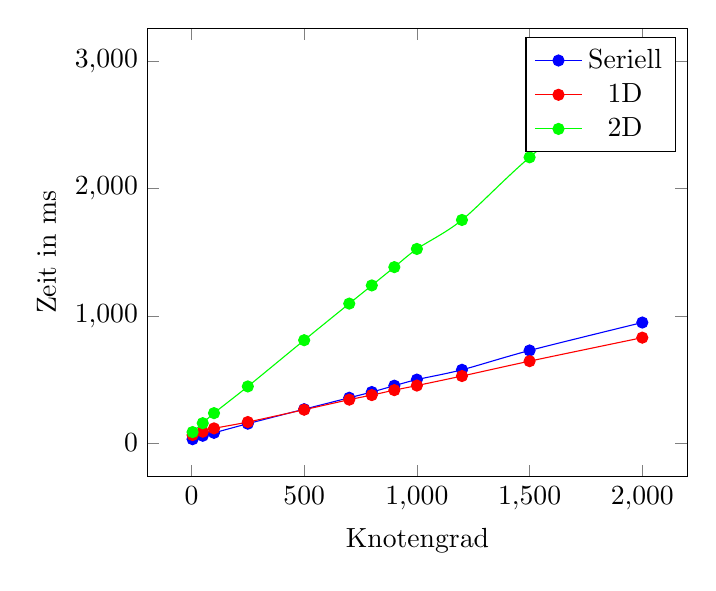
\begin{tikzpicture}
	    \begin{axis}[
	        xlabel=Knotengrad,
	        ylabel=Zeit in ms]
	    \addplot[smooth,mark=*,blue] plot coordinates {
	        (5,29)
	        (50,56)
	        (100,79)
	        (250,151)
	        (500,265)
	        (700,355)
	        (800,400)
	        (900,450)
	        (1000,498)
	        (1200,575)
	        (1500,727)
	        (2000,947)
	    };
	    \addlegendentry{Seriell}

	    \addplot[smooth,color=red,mark=*]
	        plot coordinates {
	        (5,62)
	        (50,88)
	        (100,114)
	        (250,164)
	        (500,261)
	        (700,340)
	        (800,376)
	        (900,415)
	        (1000,451)
	        (1200,526)
	        (1500,643)
	        (2000,828)
	        };
	    \addlegendentry{1D}

	    \addplot[smooth,color=green,mark=*]
	        plot coordinates {
	        (5,85)
	        (50,155)
	        (100,234)
	        (250,444)
	        (500,808)
	        (700,1096)
	        (800,1239)
	        (900,1383)
	        (1000,1526)
	        (1200,1754)
	        (1500,2247)
	        (2000, 2969)
	        };
	    \addlegendentry{2D}
	    \end{axis}
	\end{tikzpicture}
\end{figure}

\section{Ergebnisse der Parallelisierung} % (fold)
\label{sec:ergebnisse_der_parallelisierung}
Da die Breitensuche mit dem 2D Dekomposition keine vergleichbaren Ergebnisse lieferte, wird hier nur der serielle Algorithmus mit dem 1D Algorithmus verglichen. Mehr zu der 2D Breitensuche steht in Kapitel \ref{sec:die_2d_breitensuche}.
\begin{figure}
	\centering
	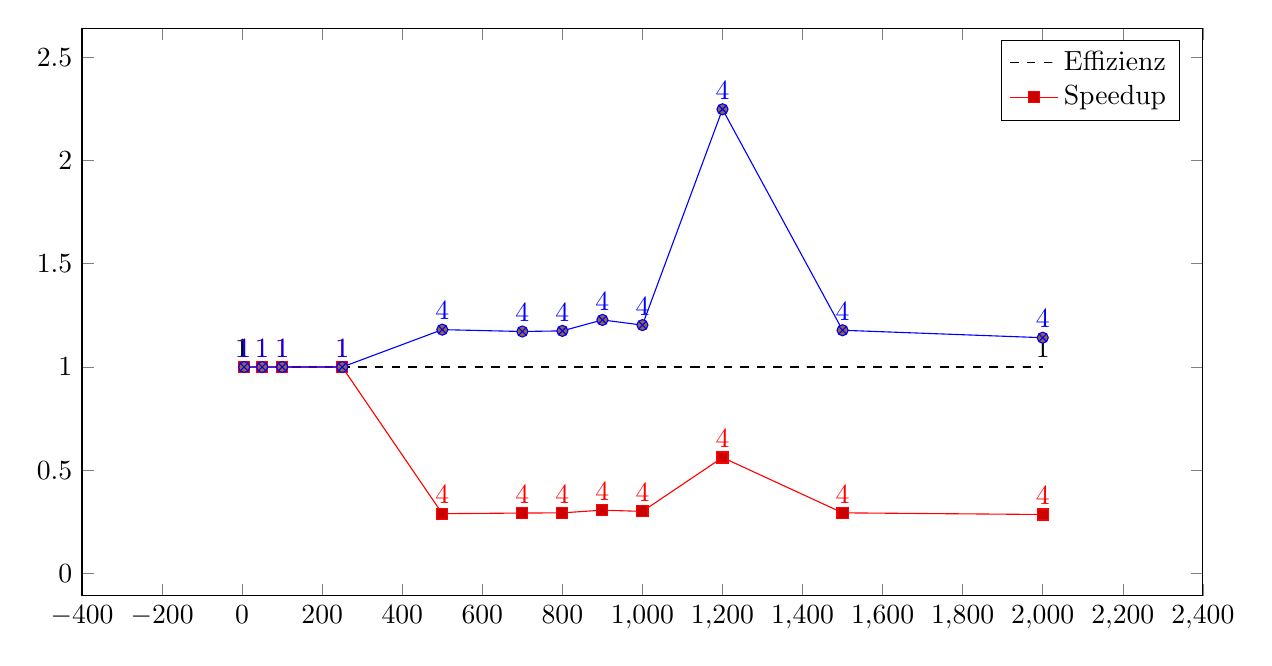
\begin{tikzpicture}
		\begin{axis}[nodes near coords,enlargelimits=0.2,width=450, height=250]
		    \addplot+[
		        smooth,
		        dashed,
		        black,
		        mark=none]
		    coordinates {
		    	(0,1)
		    	(2000,1)
		    };

		    \addplot+[red,
		        point meta=explicit symbolic]
		    coordinates {
		        (5,1) [1]
		        (50,1) [1]
		        (100,1) [1]
		        (250,1) [1]
		        (500,0.29) [4]
		        (700,0.293) [4]
		        (800,0.294) [4]
		        (900,0.307) [4]
		        (1000,0.301) [4]
		        (1200,0.562) [4]
		        (1500,0.294) [4]
		        (2000,0.286) [4]
		    };
		    \addlegendentry{Effizienz}

		    \addplot+[blue,
		        point meta=explicit symbolic]
		    coordinates {
		        (5,1) [1]
		        (50,1) [1]
		        (100,1) [1]
		        (250,1) [1]
		        (500,1.181) [4]
		        (700,1.172) [4]
		        (800,1.175) [4]
		        (900,1.228) [4]
			    (1000,1.203) [4]
			    (1200,2.248) [4]
			    (1500,1.178) [4]
			    (2000,1.142) [4]
			};
		    \addlegendentry{Speedup}

		\end{axis}
	\end{tikzpicture}
\end{figure}
% section ergebnisse_der_parallelisierung (end)

\section{Die 2D Breitensuche} % (fold)
\label{sec:die_2d_breitensuche}
Die 2D Breitensuche ist in jedem Testfall der mit Abstand langsamste Algorithmus gewesen, was so nicht zu erwarten war. Der implementierte Algorithmus ist zwar zunächst deutlich komplexer, als die anderen beiden, doch gibt es zwei Vorteile, die diesen ALgorithmus gewiss studierenswert machen. Erstens sind die Gruppen von Places, die untereinander kommunizieren deutlich kleiner. In der ersten Kommunikationsphase sendet jeder Place seine Daten an eine ganze Spalte, und empfängt dafür von einer ganzen Zeile die Daten für den nächsten Schritt. Das sind $2 * \sqrt(p)$ Places, insgesamt, mit denen jeder Place kommunizieren muss, also $O(p * 2 + \sqrt(p) * \frac{1}{2}) = O(p * \sqrt(p))= O(p^{\frac{3}{2}})$ Kommunikationsvorgänge im System. In der zweiten Kommunikationsphase muss jeweils nur eine Zeile miteinander kommunizieren. Das sind zusätzlich $O(\sqrt(p) * p * \frac{1}{2})$ Kommunikationsvorgänge. Es sind also im O-Kalkül pro Iteration $O(p^{\frac{3}{2}})$. Im Vergleich dazu kommuniziert jeder Place im 1D Algorithmus mit allen anderen p-1 Places, also $O(p^2)$ Kommunikationsvorgänge. Der zweite Vorteil der Implementierung wie in \cite{Buluc:2011} ist die Möglichkeit, alle Kommunikation und Synchronisation auf drei MPI Operationen abzubilden. Die auf entsprechender Hardware vergleichsweise schnell sind. 

Beide dieser Vorteile sind bei der X10 Implementierung, die auf nur einem CPU läuft, hinfällig. Zunächst wurden die MPI Operationen in X10 \enquote{nachprogrammiert}. Um das zu tun, muss \textit{at} verwendet werden, dass einen für diesen Zweck unnützen Rückkanal hat. Bei der Verwendung einer hochperformanten MPI Hardware muss ein Datum nur einmal gesendet werden, wenn es an mehrere Empfänger gehen soll. Das ist in X10-Syntax nicht möglich. Die zusätzliche Kommunikation ist also teurer, als sie sein müsste. 
Der zweite Vorteil, eben dass weniger Kommunikationsvorgänge im System sind, ist aus zwei Gründen hier nicht ausschlaggebend. Zum einen sind dermaßen wenig Places im Spiel, dass die Zahlen sich fast gleichen, zum anderen haben erste Tests gezeigt, dass die Kommunikationsphasen etwa 4 bis 5 Mal so schnell sind wie die Rechenphasen, also die Kommunikation nicht so ausschlaggebend ist, wie das zu erwarten war. Das wiederum ist auf die Testumgebung ohne wirklich getrennte Places zurückzuführen.

Wie in \cite{Buluc:2011} ist also die 2D Implementierung eher die schlechtere, wobei in den Dimensionen, in denen in dieser Arbeit gedacht wird,  die Unterschiede gravierender sind. Ob in  größeren Testumgebungen die Ergebnisse anders ausfallen, muss in einer weiteren Arbeit untersucht werden.
% section die_2d_breitensuche (end)
% chapter ergebnisse_und_diskussion (end)
%!TEX root = thesis.tex
\chapter{Fazit und zukünftige Arbeit} % (fold)
\label{cha:fazit_und_zuk_nftige_arbeit}

Im Rahmen dieser Arbeit konnten einige Ideen und Ansätze nicht umgesetzt werden, die womöglich in zukünftiger Arbeit anzugehen sind.

Um die bestehende Arbeit besser zu testen und um die Vor- und Nachteile besser zu verstehen, sollte der existierende Code auf einem echten Rechencluster getestet werden. Die Bedingungen unterscheiden sich stark von der parallelen Ausführung auf nur einem Prozessor. Zum einen können mit einem Rechencluster, das echten verteilten Speicher hat, wesentlich größere Graphen getestet werden. Größere Graphen bedeuten immer auch größeres Parallelisierungspotential. Zum anderen ist X10 laut den Entwicklern dafür gemacht, effiziente Programme für große verteilte Rechensysteme zu programmieren. Aus diesen zwei Gründen ist zu erwarten, dass der in dieser Arbeit erreichte Speedup weit unter dem Potential der Breitensuche geblieben ist. 

Zudem muss die Breitensuche natürlich auf der TODO Hardware getestet werden, die im Rahmen des invasIC Projekts entsteht.

Auch implementierungstechnisch gibt weitere Variationsmöglichkeiten, deren Auswirkung auf Geschwindigkeit und Beschleunigung getestet werden kann. Die einzelnen Processing Elements können auch autonomer Implementiert werden, als sie es im Moment sind. Wenn jede PE ein eigenes Intervall des Graphen bekommt und darauf autonom rechnet, würde die Synchronisation zwischen den einzelnen PEs komplett wegfallen. In der aktuellen Codebasis wäre das eine Barriere weniger. Außerdem sparte man sich die Funktionsaufrufe und die Arithmetik, um die Liste der aktiven Knoten aufzuteilen. Der Nachteil dieser Implementierung wäre, dass von einem Place zu einem anderen pro Iteration mehrere Kommunikationen stattfinden, falls mehrere PEs zum gleichen Place senden müssen. 

In der invasiven Implementierung werden im Moment keine Processing Elements abgegeben oder neu beantragt, sobald der Algorithmus einmal gestartet ist. Die Masteractivity weiß aber nach jeder Iteration, wie lang die Liste der aktiven Knoten auf jedem Place ist. Mit dieser Information könnte sie Rechenleistung freigeben oder neu beantragen. Eine entsprechende Implementierung würde die Möglichkeit des Framework nutzen, eine einmal abgegebene PE wieder zurück zu verlangen. Diese Funktion würde das in Kapitel \ref{sub:dynamische_ressourcenverwaltung} beschriebenen Problem lösen, dass anzunehmender Weise zu einem späteren Zeitpunkt genau die abgegebene Rechenleistung wieder gebraucht wird. Diese Funktionalität ist aber noch nicht vorhanden und konnte somit nicht getestet werden. 

Auch nicht getestet wurde, wie es sich ein Programm verhält, wenn die Datenhaltung auf eine veränderte Situation der Rechenleitung reagiert. Dieser Ansatz geht im Gegensatz zu dem gerade genannten davon aus, dass Rechenleistung genutzt werden soll, egal auf welchem Place sie liegt. Wenn also Rechenleistung abgegeben wurde oder neue hinzukam, müssen die Graphdaten dynamisch entsprechend an den richtigen Ort kopiert werden. Womöglich können die Daten so verteilt werden, dass ab einem gewissen Zeitpunkt für jeden Knoten mindestens zwei Places verantwortlich sind und dadurch auf weitere Änderungen sehr schnell reagiert werden kann.

% TODO: Fazit

% chapter fazit_und_zuk_nftige_arbeit (end)


%% --------------------
%% |   Bibliography   |
%% --------------------
\cleardoublepage
\nocite{*}
\phantomsection
\addcontentsline{toc}{chapter}{\bibname}

\iflanguage{english}
{\bibliographystyle{IEEEtranSA}}	% english style
{\bibliographystyle{babalpha-fl}}	% german style
												  
% Use IEEEtran for numeric references
%\bibliographystyle{IEEEtranSA})

\bibliography{thesis}


%% ----------------
%% |   Appendix   |
%% ----------------
\cleardoublepage

%!TEX root = thesis.tex
%%

%% ==============================
%\chapter{Appendix}
%\label{ch:Appendix}
%% ==============================

\appendix
\addchap{Anhang}


\section{Messwerte}
\label{Anhang-Implementierung}
Testplattform 1, alle Messwerte in ms
%!TEX root = thesis.tex
\begin{center}

\csvautotabular{Laufzeiten/100kav5.csv} \\ \vspace{1cm}
\csvautotabular{Laufzeiten/100kav50.csv} \\ \vspace{1cm}
\csvautotabular{Laufzeiten/100kav100.csv} \\ \vspace{1cm}
\csvautotabular{Laufzeiten/100kav250.csv} \\ \vspace{1cm}
\csvautotabular{Laufzeiten/100kav500.csv} \\ \vspace{1cm}
\csvautotabular{Laufzeiten/100kav700.csv} \\ \vspace{1cm}
\csvautotabular{Laufzeiten/100kav800.csv} \\ \vspace{1cm}
\csvautotabular{Laufzeiten/100kav900.csv} \\ \vspace{1cm}
\csvautotabular{Laufzeiten/100kav1000.csv} \\ \vspace{1cm}
\csvautotabular{Laufzeiten/100kav1200.csv} \\ \vspace{1cm}
\csvautotabular{Laufzeiten/100kav1500.csv} \\ \vspace{1cm}
\csvautotabular{Laufzeiten/100kav2000.csv} \\ \vspace{1cm}
\end{center}



% \setcounter{figure}{0}
		
% \begin{figure} [ht]
%   \centering
%    ein Bild
%   \caption{A figure}
%   \label{fig:BPMNBeispiela}
% \end{figure}


\end{document}
